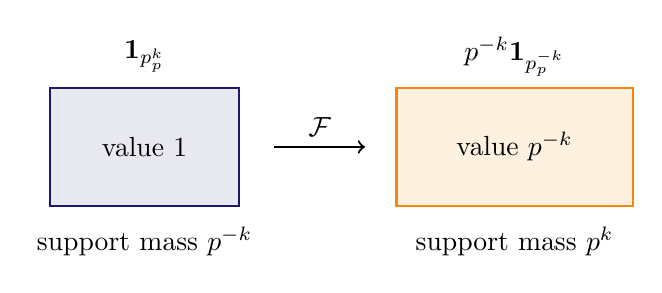
\begin{tikzpicture}[x=1cm,y=1cm]
\draw[MidnightBlue,thick,fill=MidnightBlue!10] (0,0) rectangle (2.4,1.5);
\node at (1.2,1.9) {$\mathbf1_{p^k\Z_p}$};
\node at (1.2,.75) {value $1$};
\node at (1.2,-.45) {support mass $p^{-k}$};
\draw[->,thick] (2.85,.75)--(4,.75) node[midway,above] {$\mathcal F$};
\draw[BurntOrange,thick,fill=BurntOrange!10] (4.4,0) rectangle (7.4,1.5);
\node at (5.9,1.9) {$p^{-k}\mathbf1_{p^{-k}\Z_p}$};
\node at (5.9,.75) {value $p^{-k}$};
\node at (5.9,-.45) {support mass $p^k$};
\end{tikzpicture}
